\documentclass[11pt]{article}
\usepackage[margin=1in]{geometry}
\usepackage{volfit_preamble}
\graphicspath{{figures/}}

\title{\textbf{One Straight Line}\\[2pt]
\large Forwards, discounting and dividends, told as a problem of
statistical inference\\[2pt]
\normalsize Vol-Fitter Technical Notes, No.~06}
\author{Vol-Fitter}
\date{\today}

\begin{document}
\maketitle

% Generated numbers.  fwd_tables.tex carries the original suite's band
% constants (gen_forwards.py); fwd_inference_tables.tex everything unique to
% this edition (gen_fwd_inference.py).  Never retype a generated number.
% Auto-generated by gen_forwards.py — do not edit.
\newcommand{\fwdtrue}{101.51}
\newcommand{\fwdhat}{101.51}
\newcommand{\fwdrate}{4.00}
\newcommand{\fwdratemin}{-5}
\newcommand{\fwdratemax}{30}

% Auto-generated by gen_fwd_inference.py — do not edit.
\newcommand{\fwdinfFerrbp}{0.02}
\newcommand{\fwdinfraterrbp}{0.5}
\newcommand{\fwdinfrms}{0.48}
\newcommand{\fwdinfnpairs}{20}
\newcommand{\fwdinfmcratesd}{12}
\newcommand{\fwdinfmcratepred}{11}
\newcommand{\fwdinfmcfwdsd}{0.6}
\newcommand{\fwdinfmcfwdpred}{0.6}
\newcommand{\fwdinfmcn}{400}
\newcommand{\fwdinflevernaive}{50}
\newcommand{\fwdinfleverunif}{3.2}
\newcommand{\fwdinfleverkern}{0.8}
\newcommand{\fwdinfleverkbar}{95.0}
\newcommand{\fwdinftrimrawbp}{8}
\newcommand{\fwdinftrimrawrate}{5.8}
\newcommand{\fwdinftrimbp}{0.0}
\newcommand{\fwdinftrimnout}{1}
\newcommand{\fwdinfmaskrate}{8.1}
\newcommand{\fwdinfmaskbp}{12}
\newcommand{\fwdinfmasknout}{0}
\newcommand{\fwdinfzcn}{7}
\newcommand{\fwdinfzcminrate}{-30.8}
\newcommand{\fwdinfzcmaxrate}{-0.6}
\newcommand{\fwdinfzcmedrms}{21.2}
\newcommand{\fwdinfzcmaxfdev}{1.3}
\newcommand{\fwdinfdiveq}{2.59}
\newcommand{\fwdinfdebrawbp}{46}
\newcommand{\fwdinfdebbp}{0.4}
\newcommand{\fwdinfdebrawgap}{116}
\newcommand{\fwdinfdebgap}{1}
\newcommand{\fwdinfdebrawrate}{-1.09}
\newcommand{\fwdinfdebrate}{4.74}
\newcommand{\fwdinfbsensq}{62}
\newcommand{\fwdinfbsensy}{126}
\newcommand{\fwdinfbfloory}{3}
\newcommand{\fwdinfbfloorq}{13}
\newcommand{\fwdinfbfloorwy}{16}
\newcommand{\fwdinfrefagree}{-16}
\newcommand{\fwdinfrefclrate}{-5.0}
\newcommand{\fwdinfrefclrateeq}{0.0e+00}
\newcommand{\fwdinfrefclfbp}{0}
\newcommand{\fwdinfrefrawrate}{-6.9}
\newcommand{\fwdinfgencommit}{86eba4c}
\newcommand{\fwdinfgendate}{2026-07-18}


\begin{abstract}
Every smile in this series is drawn in forward-normalized coordinates, so
before any volatility model runs, two numbers must be estimated from the
chain itself: the forward $F$ and the discount $D$.  Put--call parity makes
them the two parameters of one straight line, $C-P=D\,(F-K)$, and this
lecture reads the whole production apparatus as a single exercise in
statistical inference on that line.  Ordinary least squares identifies the
line's \emph{level} superbly and its \emph{slope} poorly --- on a realistic
chain with two-cent quote noise, the forward is pinned to a fraction of a
basis point while the implied rate wanders by tens
(\fwdinfmcratesd\ basis points measured, \fwdinfmcratepred\ predicted by
the textbook variance formula) --- and every robustness
device in production is a response to that asymmetry, matched to how the
data fails.  A residual-trim loop rejects incoherent stale quotes; an
exact lever-arm identity shows why re-deriving the forward from the
ATM-weighted price \emph{level} transmits almost none of a corrupted
slope's error (\fwdinfleverkern\ bp per percent of rate error, against
\fwdinflevernaive\ for the intercept-over-slope reading); a physical band
clamps the rate when the slope is untrustworthy; and when a delayed feed
synthesizes a chain at zero carry, the design matrix is vacuous ---
regressed on the real captured fixture it returns rates from
$\fwdinfzcminrate\%$ to $\fwdinfzcmaxrate\%$, several perfectly plausible
--- so an ingestion-time flag pins the forward to the chain's own
construction convention rather than regressing at all.  Dividends supply
the carry model (four modes, distinguished less by their term structures
than by the forward's spot-elasticity); an American de-bias removes the
early-exercise contamination of the line at a fixed point that closes the
put/call join (a raw $\fwdinfdebrawgap$-vol-bp ATM gap and
$\fwdinfdebrawbp$\,bp forward bias fall to \fwdinfdebgap\ and
\fwdinfdebbp); and the same estimation lens ends the note at the borrow
--- the carry component whose identifiability floor
(\fwdinfbfloorq\,bp at three months, \fwdinfbfloory\ at one year, per ten
basis points of quote noise) decides whether a hard-to-borrow read is a
measurement or a guess.
\end{abstract}

\newpage
\tableofcontents
\newpage

%======================================================================
\section{One straight line}
\label{sec:line}

The forward is the anchor of the whole smile.  Log-moneyness
$\logm=\log(K/F)$, the at-the-money point, the put/call OTM split, the
de-Americanization carry (Note~05) and the variance-swap replication
(Note~08) are all defined relative to $F$; the discount $D$ normalizes
every price.  An error of a fraction of a percent in $F$ shifts the ATM
strike and tilts the put--call balance, and the symptom is unmistakable: a
\emph{gap} in the at-the-money smile where the two OTM sides fail to meet.
Neither number is quoted.  Both are \emph{estimated}, from the option
prices themselves, through the one identity that European prices must
satisfy:
\begin{equation}
\boxed{\;C(K)-P(K)\;=\;D\,(F-K).\;}
\label{eq:parity}
\end{equation}
A portfolio long a call and short a put pays $S_t-K$ at expiry, a forward
contract; its price today is the discounted forward value of that payoff.
Equation~\eqref{eq:parity} is a straight line in $K$, and everything in
this note is inference on that line: the discount is (minus) its slope,
the forward is its root, and each production device below answers one
question a statistician would ask of any regression.  What do the data
identify well, and what poorly (\cref{sec:identify})?  What do outliers do
(\cref{sec:trim})?  What prior knowledge should constrain the
ill-identified direction (\cref{sec:clamp})?  When does the design contain
no information at all (\cref{sec:pin})?  What does model error --- here,
early exercise --- do to the observations (\cref{sec:debias})?  And where
is the edge beyond which a parameter, though real, is simply not
identified by the data at hand (\cref{sec:borrow})?

\begin{heuristic}
The forward is a \emph{fitted quantity with error bars}, and the two
parameters of \eqref{eq:parity} are not equally blessed.  The price
difference $C-P$ is dollars tall (its level) but changes slowly across
strikes (its slope), so the level is measured by every quote while the
slope must be teased out of small differences between them.  The design of
this note's machinery is one epistemic rule applied three times: extract
the forward where the data is informative (the level), refuse to trust
what is ill-identified (the slope, on a noisy feed), and refuse to infer
anything at all where the information is absent (a synthesized chain,
\cref{sec:pin}).
\end{heuristic}

\begin{invariant}
\begin{enumerate}[leftmargin=1.6em]
\item On a clean chain, every robustness device is byte-identical to the
plain parity regression --- the trim loop, the clamp and the de-bias
engage only on demonstrably bad inputs.
\item The implied rate never leaves a physical band; when the slope is
untrustworthy, the forward is re-derived from the well-identified price
level.
\item The discount is \emph{held} through the American de-bias --- the two
corrections never fight over the same parameter.
\item Parity is regressed only on prices that \emph{contain} parity
information: a chain synthesized from provider vols at zero carry is
flagged explicitly and pinned to its construction convention $F=S$,
$D=1$.  The flag is never inferred from zero spreads --- EOD close marks
also quote $\mathrm{bid}=\mathrm{ask}$ yet their mids carry genuine parity
information.
\item Editing a name's rate or dividends refits only that name: one
ticker's noise never touches the universe.
\end{enumerate}
\end{invariant}

\paragraph{Conventions and the notation ledger.}
$S$ is spot, $F$ the forward and $D$ the discount to expiry, $K$ a strike,
$t$ the calendar year fraction, $r=-\log(D)/t$ and $q=r-\log(F/S)/t$ the
rate and carry the pair implies.  $y(K)=C(K)-P(K)$ is the observed
call--put mid difference; $\eps$ the quote-noise standard deviation of one
mid; $n$ the number of paired strikes; $\bar K$ their mean and
$\bar K_w$ a weighted mean; $S_{KK}=\sum_i(K_i-\bar K)^2$ the design's
strike dispersion.  Hats mark estimates ($\hat F$, $\hat D$).  Dividends
are cash amounts $\delta_i$ at ex-dates $t_i$; $b$ is the borrow spread;
$\pi$ the early-exercise premium of Note~05.  One differentiation
convention: subscripted $\partial$ for partials; no primes.  One basis
point of $F$ means $10^{-4}$ relative; a vol bp is $10^{-4}$ of absolute
volatility.

\begin{table}[H]
\centering\footnotesize
\setlength{\tabcolsep}{4pt}
\begin{tabular}{@{}llll@{}}
\toprule
$S,\ F,\ D$ & spot, forward, discount &
$K,\ \bar K,\ \bar K_w,\ S_{KK}$ & strikes; means; dispersion\\[2pt]
$t,\ r,\ q$ & year fraction; implied rate, carry &
$y(K)=C-P$ & the regressed observable\\[2pt]
$\eps,\ n$ & quote-noise sd; paired strikes &
$w_i$ & level-estimator quality weights\\[2pt]
$\delta_i,\ t_i$ & cash dividends, ex-dates &
$b$ & borrow spread (carry $q=q_{\mathrm{div}}+b$)\\[2pt]
$\pi_C,\ \pi_P$ & early-exercise premia (Note~05) &
$\sigma,\ d_1$ & implied vol; Black argument\\
\bottomrule
\end{tabular}
\caption{Every symbol in the note.  Regression coefficients get no letters
of their own: the model \emph{is} $(F,D)$.}
\label{tab:ledger}
\end{table}

%======================================================================
\section{What the line identifies}
\label{sec:identify}

Fit \eqref{eq:parity} by least squares --- regress $y$ on $K$, read
$\hat D$ from the slope and $\hat F$ from the root.  In production the fit
is wrapped in the trim loop of \cref{sec:trim}, but on a clean chain the
wrapper is inert and the listing of \cref{app:ref} is the whole
algorithm.  \Cref{fig:line} runs it on the note's synthetic running
example --- $S=100$, $r=4\%$, a $1\%$ carry, six months, cent-rounded
quotes --- and recovers the forward to \fwdinfFerrbp\ bp and the rate to
\fwdinfraterrbp\ bp, with residuals at the tick scale
(\fwdinfrms\ cents RMS over \fwdinfnpairs\ paired strikes).  So far,
textbook.  The lecture starts with the question of \emph{how differently}
the two parameters are identified.

\begin{figure}[H]
\centering
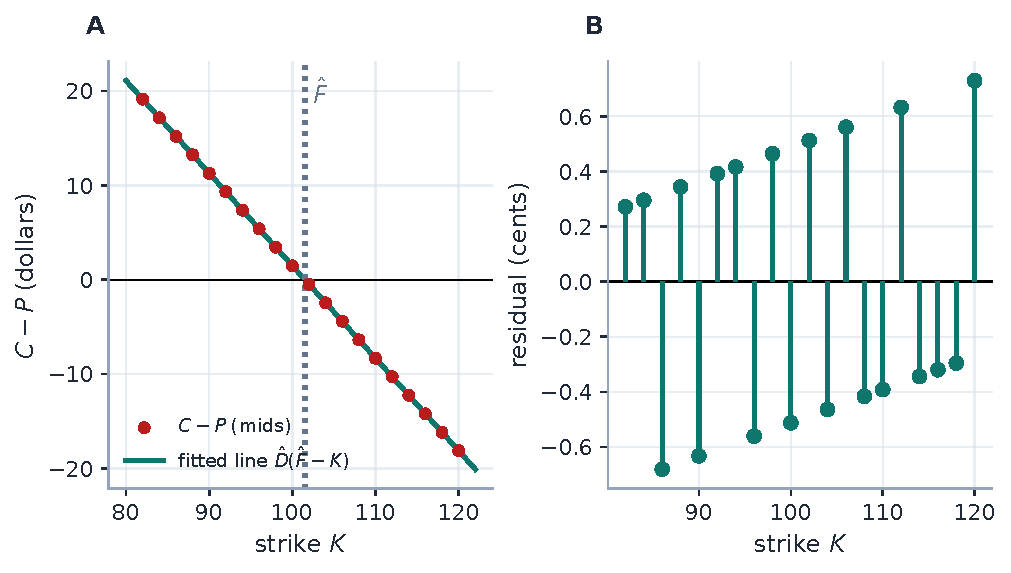
\includegraphics[width=\textwidth]{fig_fwdinf_line.pdf}
\caption{The whole estimation problem on one axis (production fit, running
example).  A: the call--put difference is a straight line in strike; its
slope is $-\hat D$, its root is $\hat F$.  B: the residuals --- cent
rounding is the only noise here, and the line comes back to \fwdinfFerrbp\
bp of forward.  Everything else in this note is about what happens to this
picture on real feeds.}
\label{fig:line}
\end{figure}

\begin{proposition}[What OLS delivers on the parity line]
\label{prop:ols}
Let each mid carry independent noise of standard deviation $\eps$, so the
difference $y$ carries $\eps\sqrt2$.  Then the least-squares estimates of
the line's \emph{slope} and of its \emph{level at $\bar K$} are
uncorrelated, with
\begin{equation}
\operatorname{sd}(\hat D)=\frac{\eps\sqrt2}{\sqrt{S_{KK}}},
\qquad
\operatorname{sd}\big(\widehat{\,y(\bar K)\,}\big)=\frac{\eps\sqrt2}{\sqrt n},
\label{eq:olssd}
\end{equation}
and the induced errors on the two market parameters separate, to first
order, as
\begin{equation}
\frac{\delta F}{F}
=\underbrace{\frac{\delta y(\bar K)}{D\,F}}_{\text{level noise}}
+\underbrace{\frac{F-\bar K}{F}\,\frac{\delta D}{D}}_{\text{slope noise}
\times\text{lever}},
\qquad
\delta r=-\frac{\delta D}{D\,t}.
\label{eq:decomp}
\end{equation}
\end{proposition}

\begin{proof}
Center the regressor: with $x=K-\bar K$ the design columns $(1,x)$ are
orthogonal, so the intercept (the level at $\bar K$) and the slope are
uncorrelated with the standard variances \eqref{eq:olssd}
\cite{SeberLee2003}.  For \eqref{eq:decomp}, write the fitted root as
$\hat F=\bar K+\hat y(\bar K)/\hat D$ (exact for OLS, in any
parametrization) and expand to first order in the two independent errors;
$\delta r$ is the chain rule on $r=-\log D/t$.
\end{proof}

Now put numbers in, because the asymmetry is the whole story.  On the
running example's design ($n=\fwdinfnpairs$ strikes spanning
$\pm20\%$), $\sqrt{S_{KK}}$ is of order fifty strike-dollars while
$\sqrt n$ is of order four --- but the slope error is then \emph{divided
by $t$} to become a rate, and multiplied only by the small lever
$F-\bar K$ to reach the forward.  The prediction: two cents of quote noise
should scatter the implied \emph{rate} by
$\approx\fwdinfmcratepred$\,bp while the \emph{forward} moves by well
under a basis point.  \Cref{fig:ident} runs \fwdinfmcn\ noisy chains
through the production estimator: measured, \fwdinfmcratesd\,bp of rate
scatter against \fwdinfmcfwdsd\,bp of forward scatter --- the formula
audited, and the design asymmetry established as fact.  The slope is the
worst-identified object in the problem; the level is nearly noiseless.
Every section that follows leans on that fact.

\begin{figure}[H]
\centering
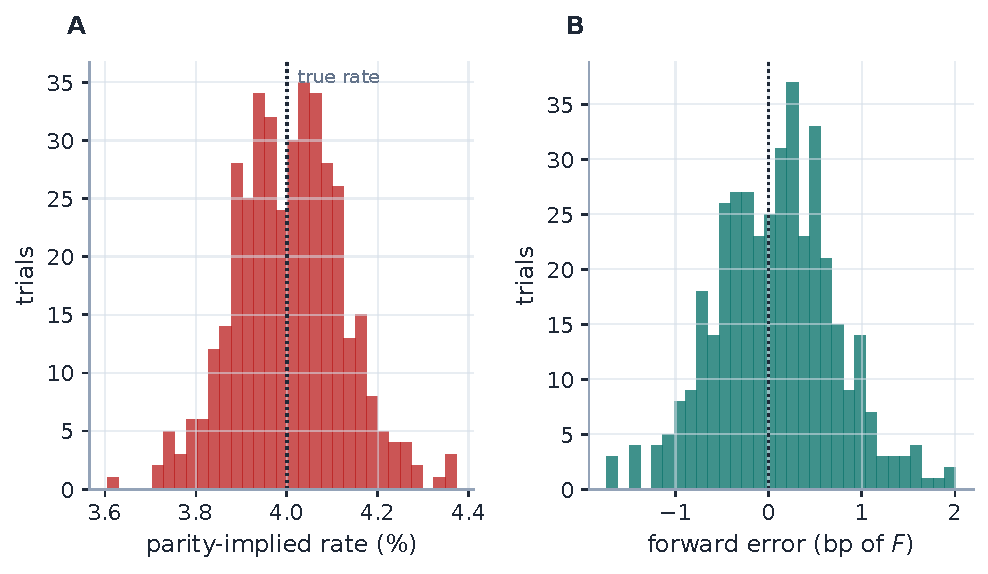
\includegraphics[width=\textwidth]{fig_fwdinf_ident.pdf}
\caption{The identifiability asymmetry, measured (\fwdinfmcn\ trials of
two-cent quote noise through the production estimator).  A: the
parity-implied \emph{rate} scatters by \fwdinfmcratesd\ bp
(\cref{prop:ols} predicts \fwdinfmcratepred).  B: the \emph{forward}
scatters by \fwdinfmcfwdsd\ bp (predicted \fwdinfmcfwdpred).  Same line,
same noise, a two-orders-of-magnitude gap in reliability: the level is
gold, the slope is lead.}
\label{fig:ident}
\end{figure}

\paragraph{Exercise 1.}
Derive the two predictions quoted above from \eqref{eq:olssd}: with
$\eps=2$ cents, $n=\fwdinfnpairs$ equally spaced strikes from $82$ to
$120$, $D\approx0.98$, $t\approx0.5$, compute
$\operatorname{sd}(\hat r)$ in basis points and
$\operatorname{sd}(\hat F)/F$ in basis points (ignore the lever term
first; then bound its contribution using $|F-\bar K|<1$).  Compare with
the measured \fwdinfmcratesd\ and \fwdinfmcfwdsd.

%======================================================================
\section{Estimating on a dirty chain}
\label{sec:trim}

Real chains carry stale and crossed quotes, and one gross point can drag a
least-squares line.  Production's answer is the classical one --- an
iterated trim: fit, form residuals, estimate a robust scale
$\hat\sigma=\max(1.4826\cdot\mathrm{median}|{\rm resid}|,\ \text{a
one-bp-of-spot floor})$, drop pairs beyond $4\hat\sigma$, refit --- at
most three rounds, never below three surviving pairs
\cite{RousseeuwLeroy1987}.  \Cref{fig:trim} stages the intended failure: a
single deep put marked \$$1.20$ stale drags the raw regression to a
$\fwdinftrimrawrate\%$ implied rate and an $\fwdinftrimrawbp$\,bp forward
error; the loop isolates the point in one round
(\fwdinftrimnout\ trimmed) and the refit recovers the truth to
\fwdinftrimbp\ bp.

\begin{figure}[H]
\centering
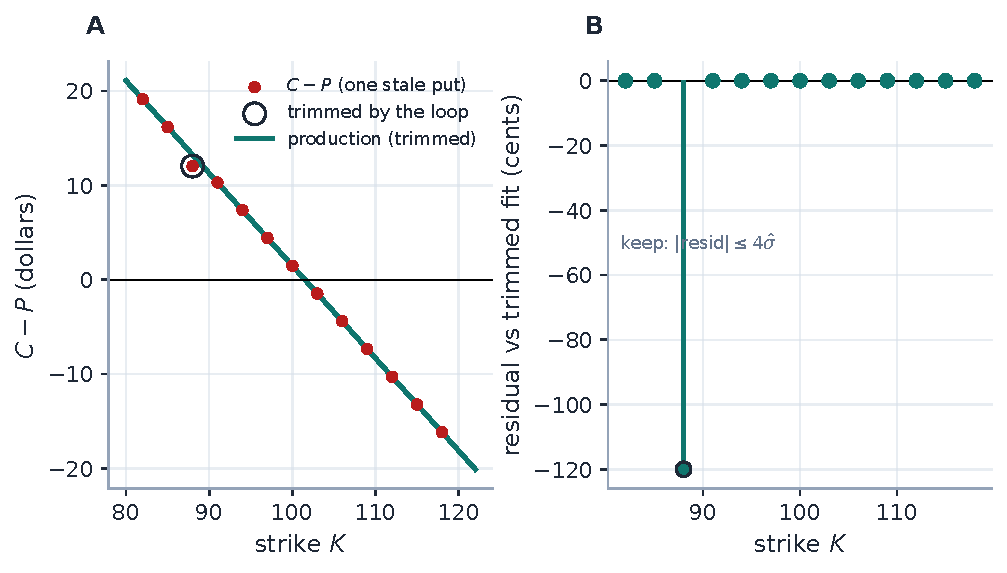
\includegraphics[width=\textwidth]{fig_fwdinf_trim.pdf}
\caption{The trim loop doing its job (production fit).  A: one grossly
stale deep put; the fitted line ignores it.  B: residuals against the
trimmed fit --- the stale quote stands $30$ robust sigmas out of a
band whose other members are at the cent scale; it is dropped in the
first round and the refit is exact to \fwdinftrimbp\ bp.  Without the
loop the same point tilts the implied rate to $\fwdinftrimrawrate\%$.}
\label{fig:trim}
\end{figure}

\begin{remark}[What the trim cannot see: coherent staleness]
\label{rem:masking}
A residual trim detects points that disagree with the consensus line.  Two
stale quotes that agree \emph{with each other} on the same wing are a
different animal: rerunning the experiment with two coherent stale puts,
the corrupted line fits them well, nothing is trimmed
(\fwdinfmasknout\ outliers flagged), and the implied rate lands at
$\fwdinfmaskrate\%$ --- \emph{inside} the physical band of
\cref{sec:clamp}, so the clamp passes it too.  This is the masking
phenomenon of robust statistics \cite{RousseeuwLeroy1987}: coherent
contamination on one wing is observationally a carry change.  What
contains the damage is \cref{prop:ols}'s asymmetry itself --- the level
stays robust, so the forward moves only \fwdinfmaskbp\ bp while the rate
absorbs the staleness.  The honest summary of the defence ladder: the trim
catches incoherent outliers, the clamp catches absurd slopes, and coherent
plausible staleness is caught by neither --- it is bounded, not fixed.
\end{remark}

%======================================================================
\section{A prior on the rate: the clamp}
\label{sec:clamp}

\Cref{sec:identify} says the slope is fragile; \cref{sec:trim} says some
failures evade the trim.  On a noisy or stale delayed feed the parity
slope drifts far enough to imply a discount above one --- a
\emph{negative} rate --- and the question is what to do when the data's
least reliable parameter contradicts prior knowledge.

\begin{caution}
A negative implied rate on a US equity chain is not a market signal; it is
feed noise sitting in the regression's worst-identified direction.
Letting it through converts a small price error into a large level error
downstream --- the discount scales every normalized price, and the tilted
slope reaches the forward through the lever of \eqref{eq:decomp}.  The
forward's level is well identified; its slope is not; treat them
accordingly.
\end{caution}

The device is Bayesian in spirit if not in ceremony: a hard prior on the
rate, $r\in[\fwdratemin\%,\fwdratemax\%]$, applied only when a reference
date pins the year fraction.  Clean chains sit strictly inside the band
and pass byte-identically (invariant~1).  When the clamp bites, the
discount is set to the band edge --- and the forward must then be
re-estimated, because $\hat F=\hat a/\hat D$ would inherit the very slope
just rejected.  Production re-derives it from the price \emph{level}: a
per-strike average of $K+y(K)/D$, weighted by quote quality (inverse
spread, floored) times a Gaussian ATM kernel of width $0.10$ in
log-moneyness.  Why that works is an identity worth isolating:

\begin{proposition}[The lever arm of a level estimator]
\label{prop:lever}
Let $\hat F_w(D')=\sum_iw_i\big(K_i+y_i/D'\big)$, $\sum w_i=1$, be a
level estimator evaluated at a possibly wrong discount $D'$.  On
noiseless data obeying \eqref{eq:parity},
\begin{equation}
\hat F_w(D')-F=\Big(1-\frac{D}{D'}\Big)\,\big(\bar K_w-F\big),
\qquad \bar K_w=\sum_iw_iK_i .
\label{eq:lever}
\end{equation}
The transmitted error is the discount error times the \emph{lever arm}
$\bar K_w-F$: where the estimator centers its strikes decides how much a
wrong discount can hurt it.
\end{proposition}

\begin{proof}
Substitute $y_i=D(F-K_i)$:
$K_i+y_i/D'=K_i(1-D/D')+F\,D/D'$, and average.
\end{proof}

Three readings of \eqref{eq:lever}, measured in \cref{fig:lever}.  The
intercept-over-slope reading $\hat F=\hat a/\hat D$ is the $w$
concentrated at $K=0$: lever $=F$ itself, and a $1\%$ rate error moves the
forward \fwdinflevernaive\ bp.  A uniform average over the board has lever
$\bar K-F$ --- small only by the accident of a balanced board
(\fwdinfleverunif\ bp per percent here, on a deliberately asymmetric one).
The production kernel centers $\bar K_w$ at the money, lever
$\approx S-F$ --- the carry itself --- and transmits
\fwdinfleverkern\ bp per percent: the forward is read where the discount
error \emph{cannot reach it}.  A final sanity bound
$|\log(F/S)|<0.5$ falls back to spot if even the level is unusable.

\begin{figure}[H]
\centering
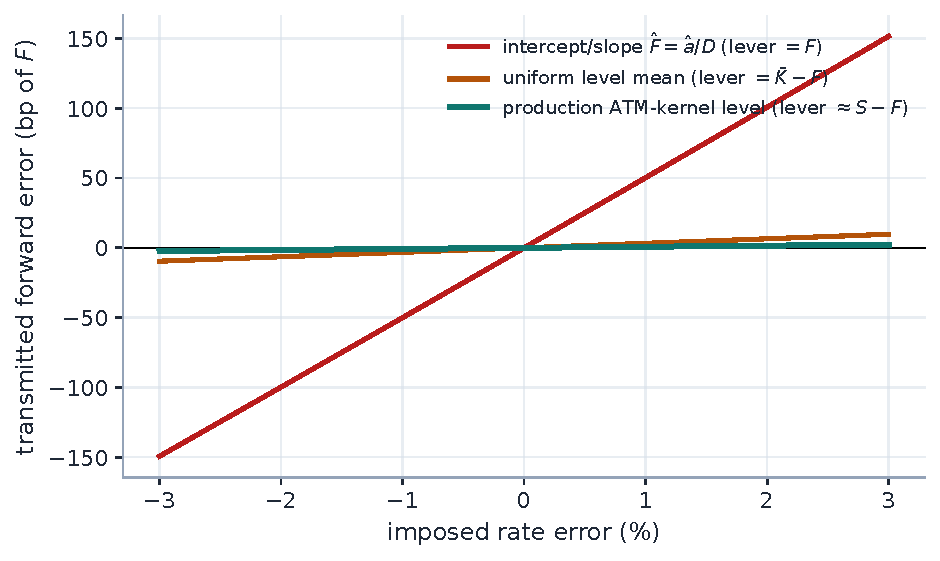
\includegraphics[width=0.8\textwidth]{fig_fwdinf_lever.pdf}
\caption{The lever-arm identity \eqref{eq:lever}, measured on an
asymmetric board.  Impose a rate error and re-derive the forward three
ways: through the intercept-over-slope reading (lever $=F$:
\fwdinflevernaive\ bp per percent of rate error), a uniform level mean
(lever $=\bar K-F$: \fwdinfleverunif), and the production ATM-kernel level
(lever $\approx S-F$: \fwdinfleverkern).  The clamp can afford to be
crude about the rate precisely because the level estimator barely feels
it.}
\label{fig:lever}
\end{figure}

\begin{example}[title={Case file: the delayed feed that gapped the ATM
smile}]
\textbf{Setup.}  Live SPY on the Massive delayed feed; also reproduced on
a Bloomberg fixture.  Quotes individually sane but collectively stale ---
mids drifting asynchronously across strikes.

\textbf{Failure.}  Parity discounts of $1.01$--$1.015$ live (up to
$1.024$ on the fixture): implied \emph{negative} rates.  The tilted slope
dragged the forward, and every ATM smile showed the telltale gap between
the put and call sides.

\textbf{The failed first fix.}  Anchoring the rate per expiry to a
smoothed term structure looked principled --- and broke everything: the
per-expiry discounts came out jagged, the LV benchmark regressed, and the
attempt deadlocked the forwards state.  Reverted.  The lesson: do not
repair an ill-identified parameter by giving it \emph{more} fitted
structure; stop trusting it.

\textbf{Fix.}  The clamp: pin the rate to the physical band, re-derive
the forward from the quality-weighted level (\cref{prop:lever}), keep
spot as the last resort.  The discount stays exactly what parity gave
whenever it is physical.

\textbf{Verdict (test-locked).}  Clean chains recover truth and pass
unclamped, byte-identical; stale-wing chains that break the raw
regression stay sane; zero-spread close-like marks still resolve; with no
reference date the clamp correctly stands down.  The residual ATM jitter
on the delayed feed is feed noise, not the forward.
\end{example}

\paragraph{Exercise 2.}
Prove the corollary used above: for the intercept-over-slope reading,
$\hat F(D')=\hat a/D'$ with $\hat a=DF$ exactly, so
$\hat F(D')-F=F\,(D/D'-1)$ --- i.e.\ \eqref{eq:lever} with
$\bar K_w=0$.  Then explain, in one sentence, why quoting options on a
\emph{forward-moneyness} grid (strikes labelled by $K/F$) would make the
uniform level mean nearly as good as the kernel one.

The clamp bounds an \emph{absurd} answer.  One failure mode remains that
it cannot see: a chain whose parity content is exactly zero, where the
regression returns wrong answers that are perfectly \emph{plausible}.
That needs its own device, and its own section.

%======================================================================
\section{A design with no information: the pin}
\label{sec:pin}

Delayed data tiers can gate the live quote stream.  When that happens the
provider does not return an empty chain --- it \emph{synthesizes} one from
its per-contract implied vols, pricing every contract with Black at
$F=S$, $D=1$, and quoting it with zero spread.  Statistically, the
resulting design is \emph{vacuous}: the forward and discount were not
observed but assumed, so the true parity content of the prices is zero.
Worse, the provider's call and put vols embed its \emph{own} carry model,
so once its contracts are re-priced at zero carry a call/put asymmetry
survives in the prices --- and a parity regression dutifully reads that
asymmetry as a forward and discount nobody ever quoted.

\Cref{fig:zerocarry} regresses the real captured fixture --- the very
chains the incident below was about --- one expiry at a time.  The
implied rates run from $\fwdinfzcminrate\%$ at the short end to
$\fwdinfzcmaxrate\%$ at a year: the shortest are absurd (the clamp would
bound them), but most sit \emph{inside} the physical band, wrong in a way
no bound can detect.  And the residuals offer no warning either: the fits
are feed-noise sized (median \fwdinfzcmedrms\ bp of spot).  A regression
cannot diagnose the vacuity of its own design from within; the only
honest detector lives \emph{upstream}, where the synthesis is known.

\begin{figure}[H]
\centering
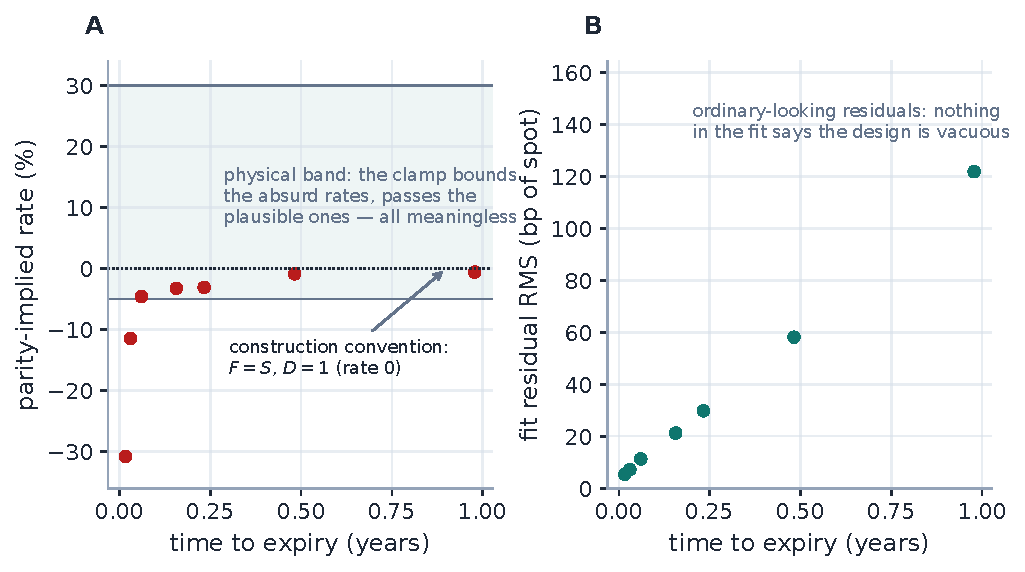
\includegraphics[width=\textwidth]{fig_fwdinf_zerocarry.pdf}
\caption{The vacuous design, on the real synthesized SPY fixture
(production regression per expiry, no pin).  A: parity-implied rates ---
all negative here, running to $\fwdinfzcminrate\%$ at the short end; the
absurd ones would be clamped, the plausible ones would pass, and
\emph{all} of them are artifacts of the provider's synthesis at $F=S$,
$D=1$.  B: the fit residuals are ordinary feed noise --- no diagnostic in
the regression says the design carries zero parity information.  The pin
answers with the only thing the chain truly contains: its construction
convention.}
\label{fig:zerocarry}
\end{figure}

\begin{example}[title={Case file: the garbage forwards the clamp could not
see}]
\textbf{Setup.}  Live SPY on the Massive delayed tier, recurring over
several sessions: the tier gated the NBBO stream, so every chain the
application received was IV-synthesized at zero carry.

\textbf{Failure.}  Recurring garbage forwards on a healthy-looking feed:
short-dated implied rates near $-4\%$, discounts above one, a one-year
forward $1.7\%$ \emph{above} the $F=S$ the prices had been built with.
The discount clamp stayed silent throughout --- the spurious rates sat
inside the physical band, so there was nothing absurd to bound.  (The
same saga's failed first fix --- the smoothed rate term structure --- is
the one already dissected in \cref{sec:clamp}.)

\textbf{Diagnosis.}  The regression was not noisy; it was answering a
question the data could not ask.  Every synthesized price is Black at
$F=S$, $D=1$, so the only structure left is the provider's call/put vol
asymmetry --- a spurious signal small enough to be plausible, which is
exactly why a clamp built for absurd slopes never fired.

\textbf{Fix.}  Recognize the regime at ingestion, not in the regression.
The provider layer flags the synthesized snapshot; for a flagged chain
the resolver returns the chain's own construction convention --- $F=S$,
$D=1$, zero residual --- and never regresses.  The flag is explicit and
persists with the snapshot, so captured chains replay correctly; it is
deliberately \emph{not} inferred from chain-wide zero spreads, because
EOD close marks also quote $\mathrm{bid}=\mathrm{ask}$ yet their mids
carry genuine parity information (invariant~4).  The Forwards tab badges
the regime so the desk knows the forward is a convention, not a market
read.

\textbf{Verdict (test-locked).}  A flagged zero-carry chain pins to
$F=S$, $D=1$ on both resolution paths; an \emph{unflagged} zero-spread
chain still regresses and recovers its true carry; the flag round-trips
through the store.  The recurring SPY forward incident is closed at the
root.
\end{example}

The pin completes an epistemic ladder that is worth stating as the
section's moral.  \emph{The regression} extracts the forward where parity
is informative; \emph{the clamp} refuses the slope where parity is noisy;
\emph{the pin} refuses the regression entirely where parity is vacuous,
returning the only honest answer the chain contains --- its own
construction convention.  The regime matters downstream too: on such
feeds anything that needs a carry (Note~05's de-Americanization, for one)
must source it externally, because the parity-implied carry is not merely
noisy but meaningless.

%======================================================================
\section{Dividends: the carry the forward carries}
\label{sec:divs}

The carry linking spot to forward must account for dividends, and the
model is per ticker, editable, and shared with the de-Americanization
tree (Note~05).  Four modes coexist.  \textbf{Discrete cash}: a schedule
of ex-dates and amounts $\delta_i$, priced by escrow ---
$F=(S-\sum_i\delta_ie^{-rt_i})\,e^{rt}$, the diffusing base being spot
minus the present value of the dividends the holder will not receive.
\textbf{Discrete proportional}: percentage haircuts per event,
$F=S\,e^{rt}\prod_i(1-\delta_i)$.  \textbf{Continuous yield}: a constant
$q$, the cheap proxy.  \textbf{Mixed}: cash for near ex-dates, switching
to a proportional treatment beyond a horizon --- the realistic
single-name default shape.  An equivalent-yield round trip across all
four modes is test-locked; on the running schedule the one-year cash leg
is worth $q_{\mathrm{eq}}=\fwdinfdiveq\%$ of continuous carry.

What distinguishes the modes is \emph{not} primarily the term structure.
\Cref{fig:divs}A shows the static picture: the cash schedule is a
sawtooth in implied carry --- violent at the short end, where one \$0.65
ex-date thirty days out annualizes to nearly $8\%$ --- against the flat
continuous proxy.  But at a fixed spot a cash schedule and a
proportional one of matching size produce nearly identical forwards; the
economic difference appears when \emph{spot moves}.  Differentiating the
escrow formula, the forward's spot elasticity is
\begin{equation}
\frac{\partial\log F}{\partial\log S}
=\frac{S}{S-\sum_i\delta_ie^{-rt_i}}\;>\;1
\quad\text{(cash)},\qquad
\frac{\partial\log F}{\partial\log S}=1\quad\text{(proportional, yield)}:
\label{eq:elasticity}
\end{equation}
cash dividends do not scale with the stock, so a rally makes the forward
outrun spot.  \Cref{fig:divs}B measures \eqref{eq:elasticity} on the
production forward by direct bump: the cash staircase climbs past $1.05$
at two years of accumulated escrow while the proportional and yield modes
sit at exactly one.  (The mixed mode's far leg re-reads its cash amounts
as fractions of the \emph{prevailing} spot, so its elasticity stays
cash-like --- a subtlety of quoting far dividends in dollars, and the
reason the mode exists is the near leg's timing, not its dynamics.)  This
elasticity is precisely what sticky-strike scenario transport
(Note~12) inherits from the dividend model, and why the mode choice is a
risk decision, not a cosmetic one.

\begin{figure}[H]
\centering
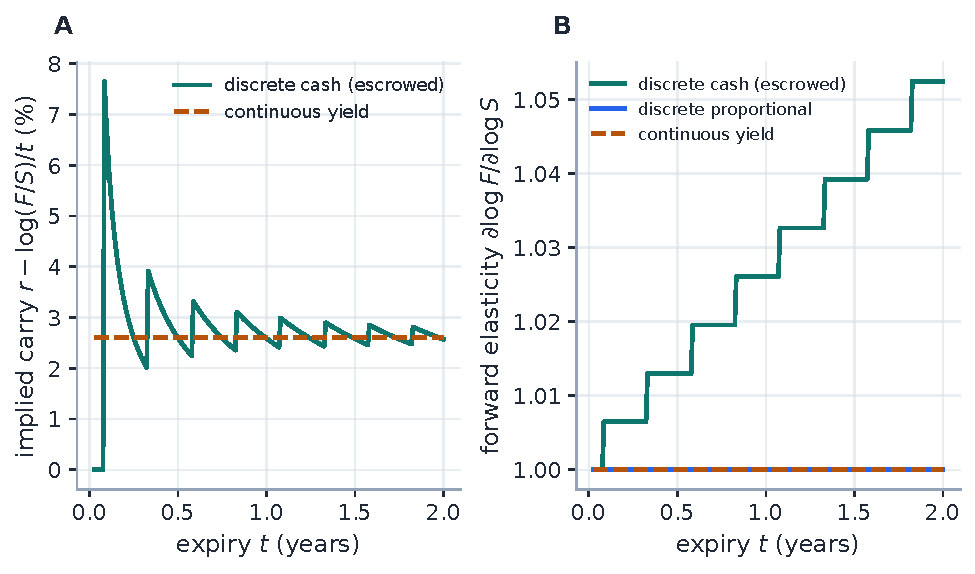
\includegraphics[width=\textwidth]{fig_fwdinf_divs.pdf}
\caption{Dividend modes, static and dynamic (production forwards, one
\$0.65-quarterly schedule).  A: the implied-carry term structure --- the
cash schedule's sawtooth against the flat continuous proxy; each tooth is
one ex-date entering the horizon.  B: the honest discriminator, the
forward's spot elasticity \eqref{eq:elasticity}: cash escrow makes the
forward outrun spot by an accumulating margin; proportional and yield
modes track it exactly.  At a fixed spot the modes look alike; on a
moving one they are different risk models.}
\label{fig:divs}
\end{figure}

%======================================================================
\section{The American de-bias}
\label{sec:debias}

For American chains the observable itself is contaminated: parity
\eqref{eq:parity} is a \emph{European} identity, but the mids on the line
are American,
\begin{equation}
y_{\mathrm{Am}}(K)=y_{\mathrm{Eu}}(K)+\pi_C(K)-\pi_P(K),
\label{eq:eiv}
\end{equation}
and the early-exercise premia $\pi_C,\pi_P$ (Note~05) are neither equal
nor constant in strike --- under positive rates the put premium dominates
and grows with $K$.  In regression language this is structured
errors-in-variables: a strike-dependent bias in the observable that
corrupts both level and slope.  The measured damage on the running
American example (a $5\%$-rate board): the raw regression's forward is
biased by \fwdinfdebrawbp\ bp and its implied rate reads
$\fwdinfdebrawrate\%$ against a true $5\%$ --- and, most visibly, the
carry error splits the de-Americanized put and call vols by
\fwdinfdebrawgap\ vol bp at the money (\cref{fig:debias}A), the ATM-kink
symptom that first motivated this machinery.

There is an apparent circularity --- de-Americanization needs the carry,
the carry comes from the forward, the forward needs de-Americanized
prices --- and production closes it as a fixed point, coarse and cheap,
with the discount \emph{held} (invariant~3).  Fixing $r=-\log D/t$ from
the raw parity: each round sets $q=r-\log(F/S)/t$ from the current
forward, de-Americanizes a near-ATM band of mids on a coarse tree,
reprices them as European, and re-implies the forward at the fixed slope
$-D$; six rounds at most, converged at a relative
$5\times10^{-5}$.  A full-depth gate then asks whether the de-Americanized
put and call vols \emph{join} at the money; if a gap above half a vol bp
per side survives, the rate itself is bisected toward the band edge until
the join closes --- the joint $(r,F)$ refinement, still inside the
physical band, still holding the parity residual as the arbiter.  On the
example the de-biased estimate recovers the forward to \fwdinfdebbp\ bp,
the rate to $\fwdinfdebrate\%$, and the ATM join to \fwdinfdebgap\ vol bp
(\cref{fig:debias}B).  Only a near-ATM band and a coarse tree enter ---
the whole refinement costs milliseconds and locates the forward to a
basis point; quote prep then runs the full-precision per-quote
de-Americanization downstream, under the refined carry (Note~05's
resolution of the same circle, seen from the other side).

\begin{figure}[H]
\centering
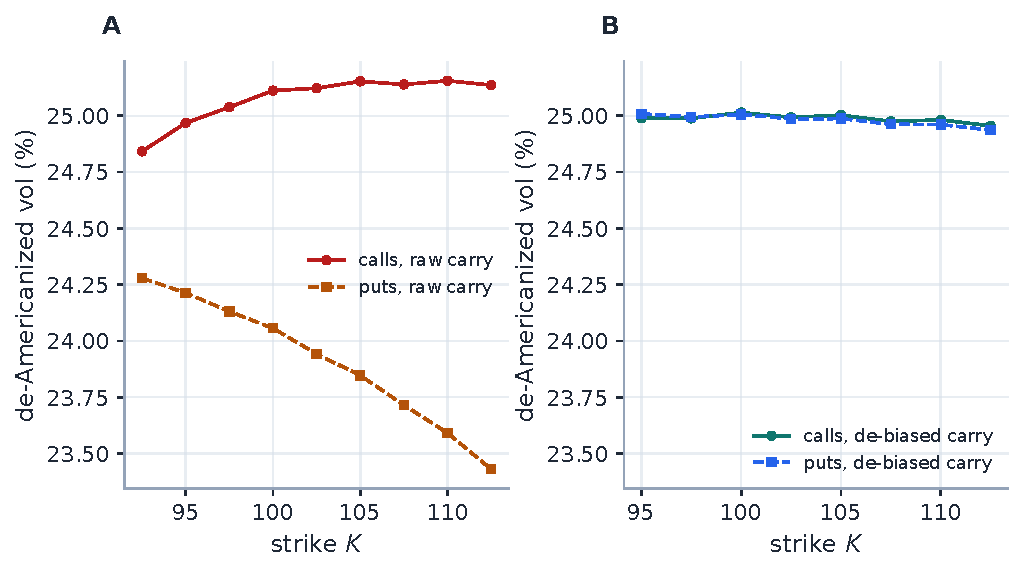
\includegraphics[width=\textwidth]{fig_fwdinf_debias.pdf}
\caption{The de-bias, before and after (production resolution on a
$5\%$-rate American board; production trees for the diagnostic).  A: at
the raw parity carry, the de-Americanized call and put vols disagree by
\fwdinfdebrawgap\ vol bp at the money and slope apart --- the ATM kink,
and a \fwdinfdebrawbp\ bp forward bias underneath it.  B: at the
de-biased carry the two sides join to \fwdinfdebgap\ vol bp on a common
flat $25\%$; the forward is recovered to \fwdinfdebbp\ bp with the
discount held throughout.}
\label{fig:debias}
\end{figure}

%======================================================================
\section{The borrow, at the edge of identifiability}
\label{sec:borrow}

The estimation lens has one more thing to say, about the carry component
this note has so far bundled silently into $q$: the \emph{borrow} $b$,
the financing spread on hard-to-borrow names,
$q=q_{\mathrm{div}}+b$.  Production carries a joint solver --- the same
fixed-point pattern as \cref{sec:debias}, iterating the borrow until the
de-Americanized, European-repriced board's parity forward matches the
theoretical forward at carry $q_{\mathrm{div}}+b$ --- but the honest
question, in this note's language, is whether $b$ is \emph{identified} at
all.  Two closed forms answer it, both shipped as diagnostics.

First, materiality.  At fixed strike and price, a borrow shift moves the
forward by $\partial F/\partial b=-tF$, and re-inverting an unchanged ATM
price moves the implied vol by
\begin{equation}
\frac{\partial\sigma}{\partial b}
=\frac{tF\cdot\partial_FC}{\partial_\sigma C}
=\frac{tF\cdot D\,\PhiN(d_1)}{D\,F\,\phin(d_1)\sqrt t}
=\sqrt t\;\frac{\PhiN(d_1)}{\phin(d_1)},
\label{eq:dsigdb}
\end{equation}
about $125\sqrt t$ vol bp per $100$ bp of borrow near the money
(\cref{fig:borrow}A): borrow uncertainty is a first-order smile input at
any maturity past a few weeks.  Second, precision.  The parity forward is
known to roughly $\mathrm{rms}/\sqrt n$ of spot
(\cref{prop:ols}'s level line), and the borrow divides that by $t$: the
\emph{noise floor}
\begin{equation}
b_{\min}\approx\frac{\mathrm{rms}/S}{t\,\sqrt n}
\label{eq:floor}
\end{equation}
is the smallest borrow the board can resolve --- \fwdinfbfloorq\ bp at
three months and \fwdinfbfloory\ bp at a year for ten basis points of
quote noise, but \fwdinfbfloorwy\ bp at a year on a fifty-bp-noise board,
and hundreds at a week on any board (\cref{fig:borrow}B).  The production
constant states its own honesty: the floor ignores the regression's
leverage on $F$, measured at another $1.5$--$2\times$ on real boards.
The conclusion \eqref{eq:dsigdb} and \eqref{eq:floor} force is the
strategic one: borrow \emph{matters} (large $\partial\sigma/\partial b$)
exactly where it may not be \emph{measurable} (floor above the
plausible borrow), and a publishable borrow read exists only where the
sensitivity-times-uncertainty product clears the floor.  That gate is
open work: on the real hard-to-borrow captures, a flat financing rate
biases the borrow one-for-one (a rate \emph{curve} is the missing input),
and held-out validation sits below thin-board noise --- measured
conclusions, recorded with the machinery, waiting on better inputs rather
than better mathematics.

\begin{figure}[H]
\centering
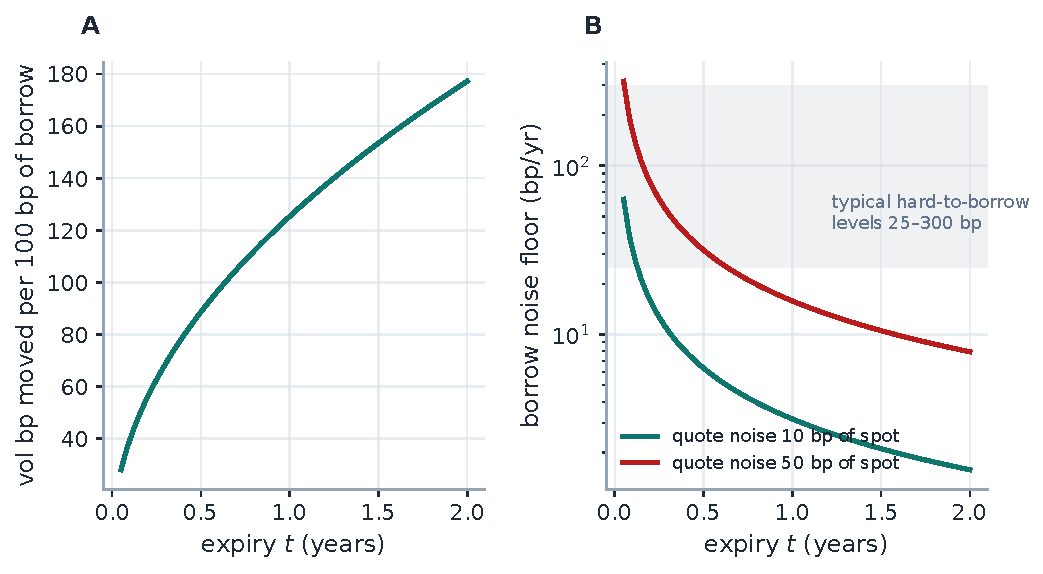
\includegraphics[width=\textwidth]{fig_fwdinf_borrow.pdf}
\caption{The borrow's two closed forms (production diagnostics).  A:
materiality --- ATM implied vol moved per $100$ bp of borrow,
\eqref{eq:dsigdb}: \fwdinfbsensq\ vol bp at three months, \fwdinfbsensy\
at a year.  B: precision --- the identifiability floor \eqref{eq:floor}
against maturity for two quote-noise levels, with typical hard-to-borrow
levels shaded: a week-dated board cannot resolve any realistic borrow; a
clean six-month board resolves tens of basis points.  A borrow read is
publishable exactly where the shaded band clears the floor.}
\label{fig:borrow}
\end{figure}

\paragraph{Exercise 3.}
From \eqref{eq:floor}: how well can a one-week expiry ($t=1/52$) with ten
paired strikes and ten basis points of quote noise pin the borrow?
(Answer: to no better than about $165$ bp --- worse than most
hard-to-borrow levels themselves.)  Conclude which expiries a borrow
term-structure read should weight, and why the joint solver's
per-expiry results must never be averaged with equal weights.

%======================================================================
\section{What is genuinely original here}
\label{sec:original}

Parity forward extraction is textbook \cite{Hull2017}; the contribution
is the estimation discipline wrapped around one straight line:
\begin{enumerate}[leftmargin=1.6em]
\item the \emph{level/slope epistemics}, made exact by
\cref{prop:ols,prop:lever} and enforced by the clamp: trust the
well-identified level, distrust the ill-identified slope, and re-derive
the forward with a lever arm of $S-F$ instead of $F$;
\item the \emph{zero-carry pin}: the recognition that a synthesized chain
is a vacuous design --- undetectable from residuals, undetectable by any
bound on plausibility --- so the regime is flagged at ingestion and the
resolver returns the construction convention rather than an estimate;
\item the \emph{de-bias fixed point} with the discount held, closing the
forward/de-Americanization circle at exactly the carry quote prep will
use, with the ATM join as the arbiter;
\item the \emph{identifiability accounting for borrow}
(\ref{eq:dsigdb}--\ref{eq:floor}): materiality and measurability computed
side by side, so an unidentified borrow is reported as such instead of
published as a number.
\end{enumerate}
All of it is byte-identical on clean data: the robustness costs nothing
when it is not needed (invariant~1).

%======================================================================
\section{Limitations}
\label{sec:limits}

Where the guarantees stop.  Parity \eqref{eq:parity} is a European
identity, and the de-bias removes the American contamination only within
Note~05's model (CRR diffusion, deterministic dividends); what the model
does not span, the fixed point cannot repair.  The clamp's band is a
prior --- correct for US equity carry today, an assumption nonetheless
--- and the coherent-staleness masking of \cref{rem:masking} passes both
trim and clamp, bounded only by the level's robustness.  The pin trusts
the provider's flag: a synthesized chain that arrives \emph{unflagged}
would be regressed in good faith (the flag's persistence and its
never-inferred-from-spreads rule are test-locked, but the upstream
detection is the provider layer's burden).  Each expiry is resolved
independently --- there is deliberately no cross-expiry smoothing after
the reverted term-structure fix, which trades away noise pooling for
robustness to one bad expiry.  And the borrow work is machinery ahead of
its inputs: a flat financing rate biases the read one-for-one, so a rate
curve --- not more iterations --- is the missing piece, and the
publishing gate stays open until held-out validation clears thin-board
noise.

\appendix
%======================================================================
\section{Hyperparameter atlas}
\label{app:atlas}

\begin{longtable}{p{0.27\textwidth}p{0.16\textwidth}p{0.49\textwidth}}
\caption{Forward/dividend/borrow hyperparameters.}\label{tab:atlas}\\
\toprule Knob & Default & Role\\ \midrule
\endfirsthead \toprule Knob & Default & Role\\ \midrule \endhead
\multicolumn{3}{l}{\emph{Surfaced}}\\ \midrule
\texttt{ForwardPolicy.mode} & \texttt{parity} & \texttt{parity}
(regression) or \texttt{theoretical} (carry model).\\
\texttt{MarketSettings.rate} $r$ & --- & Risk-free rate for the
theoretical forward / trees.\\
\texttt{dividendMode} & \texttt{continuous} & \texttt{continuous},
\texttt{discrete\_absolute}, \texttt{discrete\_proportional} or
\texttt{mixed}.\\
\texttt{dividends} / \texttt{switch\_years} & empty / $1.0$ & Discrete
$(\text{ex-date},\text{amount})$ schedule; mixed-mode horizon.\\
\texttt{jointCarry} & \texttt{false} & Gated fit-path joint borrow
(\cref{sec:borrow}); ordinary names byte-identical with the toggle on.\\
\midrule
\multicolumn{3}{l}{\emph{Hidden (parity fit / clamp)}}\\ \midrule
\texttt{RATE\_MIN/MAX} & $[\fwdratemin\%,\fwdratemax\%]$ & Physical band
for the parity-implied rate.\\
\texttt{FWD\_CLAMP\_LOG} & $0.5$ & Sanity bound on $|\log(F/S)|$; else
fall back to spot.\\
\texttt{MIN\_PAIRED\_STRIKES} & $3$ & Minimum paired strikes for a parity
fit.\\
\texttt{OUTLIER\_NSIGMA} / \texttt{MAX\_TRIM\_ROUNDS} & $4$ / $3$ &
Residual trim threshold (robust MAD scale, floored at $1$ bp of spot) and
iteration cap.\\
\texttt{ATM\_KERNEL\_H} / \texttt{SPREAD\_FLOOR\_FRAC} & $0.10$ /
$5\times10^{-4}$ & ATM kernel width and spread floor in the
level-re-derivation quality weights.\\
\midrule
\multicolumn{3}{l}{\emph{Hidden (American de-bias)}}\\ \midrule
\texttt{DEAM\_REFINE\_BAND} / \texttt{\_MAX\_STRIKES} & $0.15$ / $11$ &
Log-moneyness band and strike cap entering the fixed point.\\
\texttt{DEAM\_REFINE\_STEPS} / \texttt{\_BISECT} & $48$ / $16$ & Coarse
tree for the forward-only fixed point.\\
\texttt{MAX\_DEAM\_ITERS} / \texttt{FORWARD\_TOL\_REL} & $6$ /
$5\times10^{-5}$ & Fixed-point cap and convergence tolerance.\\
\texttt{GAP\_TOL\_VOL} / \texttt{GAP\_KERNEL\_H} & $5\times10^{-4}$ /
$0.01$ & ATM-join gate: tolerance and kernel width of the read at $F$.\\
\texttt{GAP\_TREE\_STEPS/\_BISECT} & $192$ / $24$ & Full-depth tree for
the gate and the rate bisection.\\
\texttt{GAP\_BISECT\_ITERS} / \texttt{GAP\_RATE\_TOL} & $24$ / $10^{-4}$
& Rate-bisection caps (bracket toward the band edge; sign change
required).\\
\midrule
\multicolumn{3}{l}{\emph{Hidden (joint borrow)}}\\ \midrule
\texttt{TOL} / \texttt{MAX\_ITER} & $10^{-5}$ / $8$ & Borrow fixed-point
convergence and cap.\\
\texttt{BORROW\_CAP} & $2.0$ & Hard cap on $|b|$ (200\% financing).\\
\texttt{N\_STEPS} / \texttt{BISECTIONS} & $96$ / $20$ & Coarse de-Am tree
inside the borrow loop.\\
\texttt{MIN\_PAIRS} & $6$ & Minimum call/put pairs for a borrow read.\\
\bottomrule
\end{longtable}

%======================================================================
\section{Performance notes}
\label{app:perf}

The parity regression is a $2\times2$ least squares per expiry; the trim
adds at most three refits; the clamp is a comparison.  The de-bias is a
handful of coarse-tree de-Americanizations on a near-ATM band --- about a
basis point of forward located in a few milliseconds --- and its
full-depth gate runs once, with the rate bisection engaging only when the
ATM join fails.  All are negligible against a smile fit.  Editing a
name's rate or dividend schedule bumps only that ticker's forwards
version, refitting just that name (invariant~5).  The joint borrow solver
is likewise a per-expiry fixed point over coarse trees, run as a
diagnostic column rather than on the fit path unless its toggle is on.

%======================================================================
\section{Traceability}
\label{app:trace}

\begingroup
\small
\setlength{\tabcolsep}{4pt}
\renewcommand{\arraystretch}{1.15}
\begin{longtable}{@{}p{0.42\textwidth}p{0.10\textwidth}p{0.44\textwidth}@{}}
\caption{Claims in this note and the code/tests that lock them.}\label{tab:trace}\\
\toprule Claim & Object & Code anchor \newline \emph{Test anchor}\\ \midrule
\endfirsthead
\toprule Claim & Object & Code anchor \newline \emph{Test anchor}\\ \midrule
\endhead
Clean chain: truth recovered, clamp inert (byte-identical) &
\cref{sec:clamp} &
\nolinkurl{volfit/data/forwards.py}\newline
\nolinkurl{tests/test_forward_robust.py::test_clean_chain_recovered_to_truth_and_unclamped}\\
\addlinespace
Stale wings break the raw regression; clamp stays sane &
case file &
\nolinkurl{volfit/data/forwards.py}\newline
\nolinkurl{tests/test_forward_robust.py::test_stale_wings_break_unclamped_but_clamp_stays_sane}\\
\addlinespace
Zero-spread close-like marks still resolve &
invariant~4 &
\nolinkurl{volfit/data/forwards.py}\newline
\nolinkurl{tests/test_forward_robust.py::test_zero_spread_close_like_data_still_resolves_sane}\\
\addlinespace
No reference date $\Rightarrow$ clamp stands down &
\cref{sec:clamp} &
\nolinkurl{volfit/data/forwards.py}\newline
\nolinkurl{tests/test_forward_robust.py::test_no_reference_date_skips_clamp}\\
\addlinespace
Zero-carry chain pinned to $F=S$, $D=1$ (flag decides, both paths) &
\cref{sec:pin} &
\nolinkurl{volfit/data/forwards.py}, \nolinkurl{volfit/data/types.py}\newline
\nolinkurl{tests/test_forward_robust.py::test_zero_carry_chain_pins_forward_to_spot}\\
\addlinespace
Zero spreads alone never trigger the pin &
invariant~4 &
\nolinkurl{volfit/data/types.py}\newline
\nolinkurl{tests/test_forward_robust.py::test_unflagged_zero_spread_chain_still_regresses}\\
\addlinespace
Provider flags synthesized chains; flag persists (schema v5) &
\cref{sec:pin} &
\nolinkurl{volfit/data/massive.py}, \nolinkurl{volfit/data/store.py}\newline
\nolinkurl{tests/test_massive.py::test_iv_fallback_synthesizes_fittable_chain};
\nolinkurl{tests/test_data_layer.py::test_snapshot_round_trip_keeps_zero_carry}\\
\addlinespace
Raw American board: biased forward, ATM kink &
\eqref{eq:eiv} &
\nolinkurl{volfit/data/forwards.py}\newline
\nolinkurl{tests/test_forward_debias.py::test_raw_american_forward_is_biased_and_kinks}\\
\addlinespace
De-bias holds the discount, recovers forward and rate, joins the sides &
\cref{sec:debias} &
\nolinkurl{volfit/data/forwards.py}\newline
\nolinkurl{tests/test_forward_debias.py::test_debias_recovers_discount_and_forward_and_smooths}\\
\addlinespace
Short-dated gate keeps the raw discount bit-for-bit &
\cref{sec:debias} &
\nolinkurl{volfit/data/forwards.py}\newline
\nolinkurl{tests/test_forward_debias.py::test_short_dated_chain_keeps_raw_discount}\\
\addlinespace
No localized ATM spike after de-bias; European chains unaffected &
\cref{sec:debias} &
\nolinkurl{volfit/data/forwards.py}\newline
\nolinkurl{tests/test_forward_debias.py::test_debiased_smile_has_no_localized_atm_spike};
\nolinkurl{::test_european_chain_unaffected_by_reference_date}\\
\addlinespace
0DTE: sub-day settlement horizon clamps; legacy path skips &
\cref{sec:clamp} &
\nolinkurl{volfit/data/forwards.py}\newline
\nolinkurl{tests/test_forward_robust.py::test_same_day_noisy_discount_clamped_over_subday_horizon};
\nolinkurl{::test_same_day_without_settlement_keeps_legacy_skip}\\
\addlinespace
All four dividend modes; equivalent-yield round trip &
\cref{sec:divs} &
\nolinkurl{volfit/data/dividends.py}\newline
\nolinkurl{tests/test_dividends.py::test_equivalent_yield_round_trips_every_mode};
\nolinkurl{::test_mixed_forward_switches_at_horizon}\\
\addlinespace
Joint borrow fixed point; noise floor; dIV/db &
\eqref{eq:dsigdb}, \eqref{eq:floor} &
\nolinkurl{volfit/data/carry_solve.py}\newline
\nolinkurl{tests/test_carry_solve.py}\\
\addlinespace
Per-ticker forwards version scoping &
invariant~5 &
\nolinkurl{volfit/api/state.py}\newline
\nolinkurl{tests/test_api_forwards.py::test_parity_defaults_cover_the_ladder}\\
\bottomrule
\end{longtable}
\endgroup

%======================================================================
\section{Reference implementations}
\label{app:ref}

Two listings, both executed against production by this edition's
generator before the note was committed.  The parity regression below
reproduces the production fit on the clean running example to
$10^{\fwdinfrefagree}$ (floating-point identity; production wraps the
same least squares in the trim loop, inert on clean data).  The clamp
listing reproduces production's clamped \emph{rate} exactly on the
tilted-board demo (raw rate $\fwdinfrefrawrate\%$, clamped to
$\fwdinfrefclrate\%$, agreement $\fwdinfrefclrateeq$) and its re-derived
forward to \fwdinfrefclfbp\ bp --- the production version replaces the
uniform mean with the quality-weighted, spot-fallback-guarded
\cref{prop:lever} estimator, which on this symmetric board is the same
number to under a basis point.

\begin{lstlisting}[caption={Put--call parity regression for the forward and
discount --- distilled from \texttt{data/forwards.py} (production uses
\texttt{lstsq} inside the outlier-trim loop and takes the snapshot, not
raw arrays).},label={lst:parity}]
def implied_forward(K, call_mid, put_mid):
    y = call_mid - put_mid              # C - P = D F - D K
    b, a = np.polyfit(K, y, 1)          # slope = -D, intercept = D F
    D = -b                              # discount factor
    return a/D, D                       # forward F = a/D
\end{lstlisting}

\begin{lstlisting}[caption={The discount clamp and level re-derivation ---
simplified from \texttt{data/forwards.py}, where the level mean is the
quality-weighted \texttt{\_forward\_at\_discount} (inverse spread
$\times$ ATM kernel) with the spot fallback of \cref{sec:clamp}.}]
def clamp_forward(K, call_mid, put_mid, t, F, D, r_lo=-0.05, r_hi=0.30):
    r = -np.log(D)/t                     # the parity slope's implied rate
    if r_lo <= r <= r_hi:
        return F, D                      # physical: keep the regression result
    D = np.exp(-np.clip(r, r_lo, r_hi)*t)         # clamp the rate to the band
    F = np.mean(K + (call_mid - put_mid)/D)       # re-derive F from the LEVEL
    return F, D                                   #   (lever K.bar - F, Prop. 2)
\end{lstlisting}

\begin{thebibliography}{9}
\bibitem{Hull2017} J.~Hull.  \emph{Options, Futures, and Other
Derivatives}.  Pearson, 10th ed., 2017.
\bibitem{Gatheral2006} J.~Gatheral.  \emph{The Volatility Surface}.
Wiley, 2006.
\bibitem{SeberLee2003} G.~Seber and A.~Lee.  \emph{Linear Regression
Analysis}.  Wiley, 2nd ed., 2003.
\bibitem{RousseeuwLeroy1987} P.~Rousseeuw and A.~Leroy.  \emph{Robust
Regression and Outlier Detection}.  Wiley, 1987.
\end{thebibliography}

\end{document}
